This chapter reports answer quality, operational failure detection, and their relationship across the three datasets. All bounded values are displayed as percentages and differences as percentage points; calculations remain on standard normalised scales. Results are descriptive because one inference run is available and no confidence intervals or significance tests were calculated.

\section{Overall Experimental Results}

Table~\ref{tab:overall-result-pattern} summarises the central result. PathVQA gives a metric-dependent answer ranking: Qwen2.5-VL-3B-Instruct leads BLEU-1 and BLEU-2, while MedGemma-4B-it leads ROUGE-L and METEOR; Qwen2.5-VL-3B-Instruct has the highest detector AUROC. VQA-RAD shows clearer divergence because MedGemma-4B-it leads three answer metrics but Qwen2.5-VL-3B-Instruct leads failure detection. ProstateMM-CHIMERA instead shows alignment, with MedGemma-4B-it leading three answer metrics and AUROC. The relationship is therefore not constant across metrics or datasets, and the small patient-linked prostate result requires particular caution.

\begin{table}[htbp]
    \centering
    \caption{Central comparison between answer quality and failure detection.}
    \label{tab:overall-result-pattern}
    \small
    \begin{tabularx}{\textwidth}{lXXrl}
        \toprule
        Dataset & Answer-quality leader & Best detector (model; method) & AUROC & Relationship \\
        \midrule
        PathVQA & Qwen2.5-VL-3B-Instruct on BLEU; MedGemma-4B-it on ROUGE-L/METEOR & Qwen2.5-VL-3B-Instruct; question-aligned & 81.20\% & Metric-dependent \\
        VQA-RAD & MedGemma-4B-it on three metrics & Qwen2.5-VL-3B-Instruct; Semantic AFD & 69.43\% & \textbf{Divergent} \\
        ProstateMM-CHIMERA & MedGemma-4B-it on three metrics & MedGemma-4B-it; question-aligned & 93.88\% & \textbf{Aligned} \\
        \bottomrule
    \end{tabularx}
\end{table}

\section{Answer Quality on PathVQA}

Table~\ref{tab:answer-quality-all} shows all answer results. On PathVQA, Qwen2.5-VL-3B-Instruct leads BLEU-1 at 25.29\% and BLEU-2 at 1.38\%, whereas MedGemma-4B-it leads ROUGE-L at 34.77\% and METEOR at 17.73\%; LLaVA-1.5-7B is lowest on all four metrics. Relative to Qwen2.5-VL-3B-Instruct, MedGemma-4B-it is 3.03 percentage points higher on ROUGE-L and 1.63 points higher on METEOR but 5.78 points lower on BLEU-1 and 0.95 points lower on BLEU-2. Answer strength on this dataset therefore depends on the metric, so all four measures are retained rather than combined into one accuracy value.

\begin{table}[htbp]
    \centering
    \caption{Answer-quality comparison. Bold and underlined values are best and second-best within each dataset and metric.}
    \label{tab:answer-quality-all}
    \begin{tabularx}{\textwidth}{lXrrrr}
        \toprule
        Dataset & Model & BLEU-1 & BLEU-2 & ROUGE-L & METEOR \\
        \midrule
        \multirow{3}{*}{PathVQA}
        & Qwen2.5-VL-3B-Instruct & \textbf{25.29\%} & \textbf{1.38\%} & \underline{31.74\%} & \underline{16.10\%} \\
        & LLaVA-1.5-7B & \underline{19.89\%} & \underline{0.74\%} & 26.75\% & 13.53\% \\
        & MedGemma-4B-it & 19.51\% & 0.43\% & \textbf{34.77\%} & \textbf{17.73\%} \\
        \midrule
        \multirow{3}{*}{VQA-RAD}
        & Qwen2.5-VL-3B-Instruct & \underline{39.37\%} & \textbf{8.49\%} & \underline{48.16\%} & \underline{25.94\%} \\
        & LLaVA-1.5-7B & 38.41\% & 4.88\% & 40.25\% & 20.42\% \\
        & MedGemma-4B-it & \textbf{40.18\%} & \underline{6.60\%} & \textbf{58.66\%} & \textbf{31.05\%} \\
        \midrule
        \multirow{3}{*}{ProstateMM-CHIMERA}
        & Qwen2.5-VL-3B-Instruct & \underline{25.54\%} & \underline{8.77\%} & \underline{19.56\%} & \textbf{22.48\%} \\
        & LLaVA-1.5-7B & 19.00\% & 2.18\% & 15.27\% & 13.90\% \\
        & MedGemma-4B-it & \textbf{62.24\%} & \textbf{28.57\%} & \textbf{21.86\%} & \underline{16.77\%} \\
        \bottomrule
    \end{tabularx}
\end{table}

\section{Answer Quality on VQA-RAD}

On VQA-RAD, MedGemma-4B-it leads BLEU-1, ROUGE-L, and METEOR, while Qwen2.5-VL-3B-Instruct leads BLEU-2 and LLaVA-1.5-7B is lowest throughout. MedGemma-4B-it's ROUGE-L of 58.66\% is 10.50 percentage points above Qwen2.5-VL-3B-Instruct and 18.41 points above LLaVA-1.5-7B. Its METEOR of 31.05\% is also highest. These within-dataset rankings support MedGemma-4B-it as the strongest answer generator on three measures, but higher absolute values than PathVQA do not prove that radiology is easier because answer style and reference distributions differ.

\section{Operational Failure Distribution}

The final per-record exports allow the operational failure prevalence to be reported for the complete test splits. These values are the proportion of records whose greedy answer falls below both fixed reference-matching thresholds; they are not clinical error rates. MedGemma-4B-it has the lowest prevalence on all three datasets, while Qwen2.5-VL-3B-Instruct has a lower prevalence than LLaVA-1.5-7B on VQA-RAD. This describes failure burden, not detector quality: a model can produce fewer metric-defined failures without ranking its remaining failures well. AUPRC is interpreted cautiously because it also depends on positive-class prevalence.

\begin{table}[htbp]
    \centering
    \caption{Operational failure prevalence in the complete test split. Values are percentages of all evaluated records and are not clinical error rates.}
    \label{tab:failure-prevalence}
    \begin{tabularx}{\textwidth}{lXrr}
        \toprule
        Dataset & Model & Test records & Failure prevalence \\
        \midrule
        PathVQA & Qwen2.5-VL-3B-Instruct & 6,719 & \underline{66.88\%} \\
        PathVQA & LLaVA-1.5-7B & 6,719 & 71.96\% \\
        PathVQA & MedGemma-4B-it & 6,719 & \textbf{62.94\%} \\
        VQA-RAD & Qwen2.5-VL-3B-Instruct & 451 & \underline{47.23\%} \\
        VQA-RAD & LLaVA-1.5-7B & 451 & 58.09\% \\
        VQA-RAD & MedGemma-4B-it & 451 & \textbf{36.81\%} \\
        ProstateMM-CHIMERA & Qwen2.5-VL-3B-Instruct & 42 & 54.76\% \\
        ProstateMM-CHIMERA & LLaVA-1.5-7B & 42 & \underline{42.86\%} \\
        ProstateMM-CHIMERA & MedGemma-4B-it & 42 & \textbf{33.33\%} \\
        \bottomrule
    \end{tabularx}
\end{table}

\section{Failure Detection Results}

On PathVQA, Qwen2.5-VL-3B-Instruct has the highest AUROC for every informed detector and reaches 81.20\% with question-aligned uncertainty (Table~\ref{tab:pathvqa-failure-detection}). AFD frequency is best by AUROC for LLaVA-1.5-7B at 69.55\% and MedGemma-4B-it at 68.63\%, whereas question-aligned uncertainty gives their highest AUPRC. Random AUROCs remain close to 50\%. At 50\% coverage, all selected best-AUROC conditions improve accepted ROUGE-L and reduce failure rate relative to random ranking (Table~\ref{tab:selective-gain-50}); the largest PathVQA change is Qwen2.5-VL-3B-Instruct, with ROUGE-L rising by 21.65 points and failure rate falling by 21.52 points.

\begin{table}[htbp]
    \centering
    \caption{Retained failure detectors on PathVQA. Bold and underlined values are best and second-best within each model.}
    \label{tab:pathvqa-failure-detection}
    \begin{tabularx}{\textwidth}{XXrr}
        \toprule Model & Detector & AUROC & AUPRC \\ \midrule
        Qwen2.5-VL-3B-Instruct & Question-aligned uncertainty & \textbf{81.20\%} & \textbf{90.71\%} \\
        Qwen2.5-VL-3B-Instruct & AFD frequency & \underline{79.38\%} & \underline{86.08\%} \\
        Qwen2.5-VL-3B-Instruct & Semantic AFD & 78.59\% & 85.61\% \\
        Qwen2.5-VL-3B-Instruct & Random baseline & 50.91\% & 66.78\% \\ \midrule
        LLaVA-1.5-7B & Question-aligned uncertainty & 64.76\% & \textbf{83.39\%} \\
        LLaVA-1.5-7B & AFD frequency & \textbf{69.55\%} & \underline{82.93\%} \\
        LLaVA-1.5-7B & Semantic AFD & \underline{66.06\%} & 80.97\% \\
        LLaVA-1.5-7B & Random baseline & 50.14\% & 71.78\% \\ \midrule
        MedGemma-4B-it & Question-aligned uncertainty & 62.96\% & \textbf{77.92\%} \\
        MedGemma-4B-it & AFD frequency & \textbf{68.63\%} & \underline{75.61\%} \\
        MedGemma-4B-it & Semantic AFD & \underline{64.17\%} & 72.73\% \\
        MedGemma-4B-it & Random baseline & 50.42\% & 62.87\% \\ \bottomrule
    \end{tabularx}
\end{table}

\begin{table}[htbp]
    \centering
    \caption{Gain over random ranking at 50\% coverage. Positive percentage-point values are favourable.}
    \label{tab:selective-gain-50}
    \small
    \begin{tabularx}{\textwidth}{lXXrr}
        \toprule Dataset & Model & Best detector & $\Delta$ROUGE-L & Failure-rate reduction \\ \midrule
        PathVQA & Qwen2.5-VL-3B-Instruct & Question-aligned & \textbf{21.65\%} & \textbf{21.52\%} \\
        PathVQA & LLaVA-1.5-7B & AFD frequency & 10.89\% & 10.32\% \\
        PathVQA & MedGemma-4B-it & AFD frequency & 12.79\% & 11.88\% \\ \midrule
        VQA-RAD & Qwen2.5-VL-3B-Instruct & Semantic AFD & \textbf{12.48\%} & \textbf{11.51\%} \\
        VQA-RAD & LLaVA-1.5-7B & Semantic AFD & 8.09\% & 7.07\% \\
        VQA-RAD & MedGemma-4B-it & Question-aligned & 3.11\% & 4.87\% \\ \midrule
        ProstateMM-CHIMERA & Qwen2.5-VL-3B-Instruct & Question-aligned & 6.13\% & 14.28\% \\
        ProstateMM-CHIMERA & LLaVA-1.5-7B & Question-aligned & 7.26\% & \textbf{28.57\%} \\
        ProstateMM-CHIMERA & MedGemma-4B-it & Question-aligned & \textbf{11.68\%} & \textbf{28.57\%} \\ \bottomrule
    \end{tabularx}
\end{table}

Figures~\ref{fig:performance-rejection-qwen}--\ref{fig:performance-rejection-medgemma} show that informed detectors usually improve PathVQA accepted ROUGE-L as exclusion increases. On ProstateMM-CHIMERA, question-aligned uncertainty improves all three models, whereas AFD frequency can perform below random for Qwen2.5-VL-3B-Instruct and LLaVA-1.5-7B, supporting dataset-specific detector selection.

\begin{figure}[htbp]
    \centering
    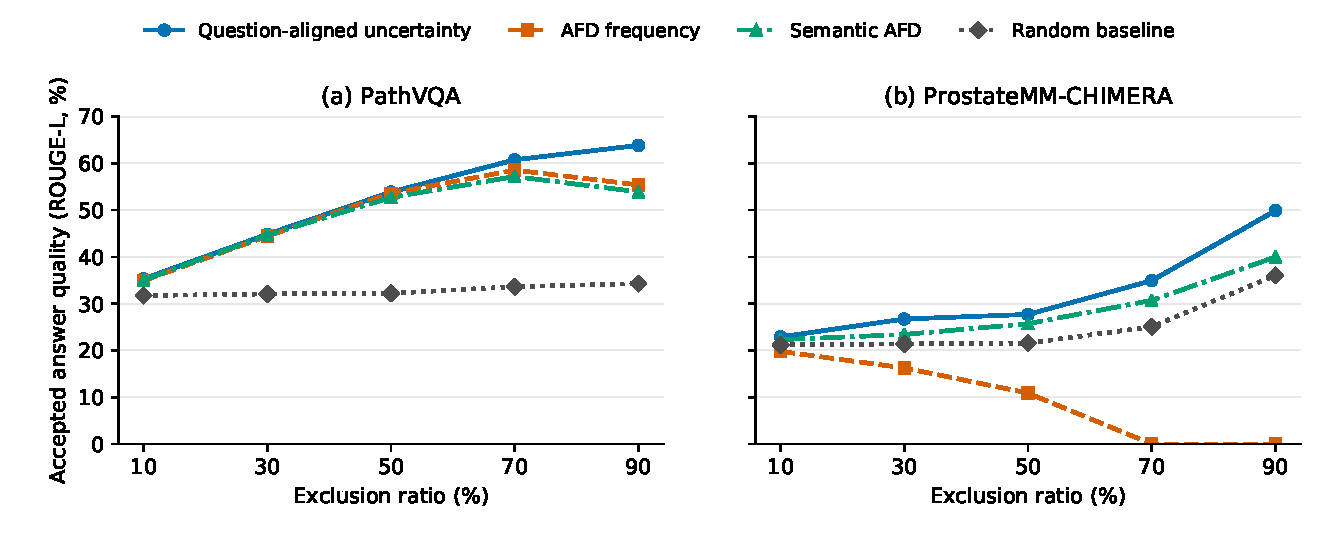
\includegraphics[width=0.92\textwidth]{Images/performance_rejection_qwen.pdf}
    \caption{Accepted ROUGE-L by exclusion for Qwen2.5-VL-3B-Instruct on PathVQA and ProstateMM-CHIMERA.}
    \label{fig:performance-rejection-qwen}
\end{figure}

\begin{figure}[htbp]
    \centering
    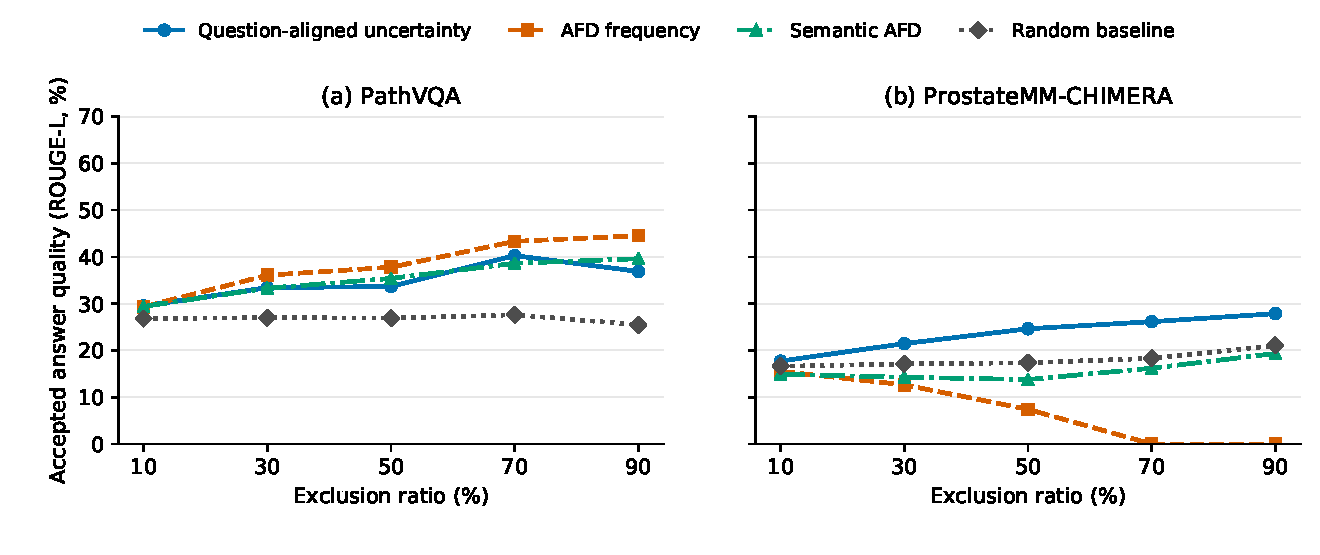
\includegraphics[width=0.92\textwidth]{Images/performance_rejection_llava.pdf}
    \caption{Accepted ROUGE-L by exclusion for LLaVA-1.5-7B on PathVQA and ProstateMM-CHIMERA.}
    \label{fig:performance-rejection-llava}
\end{figure}

\begin{figure}[htbp]
    \centering
    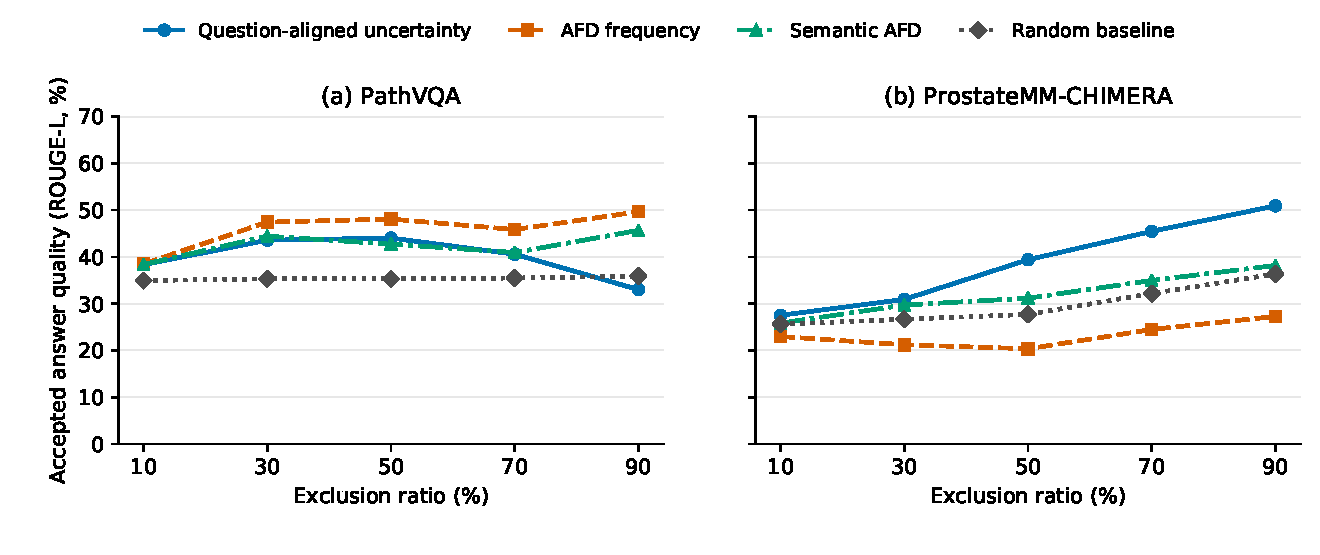
\includegraphics[width=0.92\textwidth]{Images/performance_rejection_medgemma.pdf}
    \caption{Accepted ROUGE-L by exclusion for MedGemma-4B-it on PathVQA and ProstateMM-CHIMERA.}
    \label{fig:performance-rejection-medgemma}
\end{figure}

\section{Model Ranking Across Dimensions}

Table~\ref{tab:best-detector-all} gives the best detector for every model and dataset. PathVQA ranks Qwen2.5-VL-3B-Instruct, LLaVA-1.5-7B, then MedGemma-4B-it by AUROC, agreeing with BLEU but conflicting with ROUGE-L and METEOR. The clearest contrast is between Qwen2.5-VL-3B-Instruct and MedGemma-4B-it: MedGemma-4B-it leads the latter answer metrics, yet Qwen2.5-VL-3B-Instruct's best AUROC is 12.57 percentage points higher. LLaVA-1.5-7B also has the lowest answer scores but a slightly higher PathVQA AUROC than MedGemma-4B-it. Average answer quality therefore does not determine failure ranking.

\begin{table}[htbp]
    \centering
    \caption{Best retained detector for each model and dataset.}
    \label{tab:best-detector-all}
    \begin{tabularx}{\textwidth}{lXXrr}
        \toprule Dataset & Model & Best detector & AUROC & AUPRC \\ \midrule
        PathVQA & Qwen2.5-VL-3B-Instruct & Question-aligned & \textbf{81.20\%} & \textbf{90.71\%} \\
        PathVQA & LLaVA-1.5-7B & AFD frequency & \underline{69.55\%} & \underline{82.93\%} \\
        PathVQA & MedGemma-4B-it & AFD frequency & 68.63\% & 75.61\% \\ \midrule
        VQA-RAD & Qwen2.5-VL-3B-Instruct & Semantic AFD & \textbf{69.43\%} & \underline{69.52\%} \\
        VQA-RAD & LLaVA-1.5-7B & Semantic AFD & 63.67\% & \textbf{73.53\%} \\
        VQA-RAD & MedGemma-4B-it & Question-aligned & \underline{66.03\%} & 61.47\% \\ \midrule
        ProstateMM-CHIMERA & Qwen2.5-VL-3B-Instruct & Question-aligned & 81.69\% & \underline{87.59\%} \\
        ProstateMM-CHIMERA & LLaVA-1.5-7B & Question-aligned & \underline{87.27\%} & 86.12\% \\
        ProstateMM-CHIMERA & MedGemma-4B-it & Question-aligned & \textbf{93.88\%} & \textbf{89.59\%} \\ \bottomrule
    \end{tabularx}
\end{table}

\section{Overall Validation}

VQA-RAD confirms divergence: MedGemma-4B-it leads three answer metrics, but Qwen2.5-VL-3B-Instruct has the highest AUROC at 69.43\%. At 50\% coverage, its Semantic AFD raises accepted ROUGE-L from 48.07\% to 60.55\% and lowers failure rate from 47.35\% to 35.84\%. ProstateMM-CHIMERA reverses the pattern: MedGemma-4B-it leads three answer metrics and failure detection at 93.88\% AUROC; its question-aligned detector raises accepted ROUGE-L from 27.71\% to 39.39\% and reduces the 50\%-coverage failure rate from 28.57\% to 0.00\%. This aligned result is based on only 21 accepted task records. Detector choice also changes across settings, so neither a model nor a method is uniformly dominant.

\section{Representative Quantitative Cases}

Table~\ref{tab:representative-quantitative-cases} provides one verified 50\%-coverage case per dataset using aggregate outputs. Each informed detector improves accepted ROUGE-L and lowers failure rate relative to an equally sized random subset. The PathVQA case gives gains of 21.65 and 21.52 percentage points, VQA-RAD gives 12.48 and 11.51 points, and ProstateMM-CHIMERA gives an 11.68-point ROUGE-L gain and a 28.57-point failure-rate reduction. These are quantitative operating-point cases, not individual clinical examples; item-level images and answers will be reported only if complete scored records can be verified.

\begin{table}[htbp]
    \centering
    \caption{Representative quantitative cases at 50\% coverage; arrows show random to selected-detector results.}
    \label{tab:representative-quantitative-cases}
    \small
    \begin{tabularx}{\textwidth}{lXrrr}
        \toprule Dataset & Model and detector & Records & Accepted ROUGE-L & Failure rate \\ \midrule
        PathVQA & Qwen2.5-VL-3B-Instruct; question-aligned & 3,360 & 32.20\% $\rightarrow$ 53.85\% & 66.40\% $\rightarrow$ 44.88\% \\
        VQA-RAD & Qwen2.5-VL-3B-Instruct; Semantic AFD & 226 & 48.07\% $\rightarrow$ 60.55\% & 47.35\% $\rightarrow$ 35.84\% \\
        ProstateMM-CHIMERA & MedGemma-4B-it; question-aligned & 21 & 27.71\% $\rightarrow$ 39.39\% & 28.57\% $\rightarrow$ 0.00\% \\ \bottomrule
    \end{tabularx}
\end{table}

\section{Hypothesis and Objective Support}

Table~\ref{tab:hypothesis-support} links the planned hypotheses to the evidence reported in this chapter. The support is descriptive: the study uses one inference run, one seed, and a metric-defined failure endpoint, so the table does not represent statistical confirmation or clinical validation.

\begin{table}[htbp]
    \centering
    \caption{Support for the study hypotheses and linked objectives.}
    \label{tab:hypothesis-support}
    \small
    \begin{tabularx}{\textwidth}{>{\raggedright\arraybackslash}p{3.1cm}XX>{\raggedright\arraybackslash}p{2.1cm}}
        \toprule
        Hypothesis or objective & Evidence used & Main result & Interpretation \\
        \midrule
        H1: answer quality and failure awareness can diverge & Answer-quality and detector rankings across datasets & VQA-RAD and PathVQA show different leaders, while ProstateMM-CHIMERA is aligned & Supported conditionally \\
        H2: detector performance depends on model and dataset & AUROC/AUPRC comparison for three models and four retained methods & The best detector changes across model--dataset pairs & Supported descriptively \\
        H3: informative detection improves selective operation & Accepted ROUGE-L and failure rate at matched coverage & Selected detectors improve the 50\% operating point relative to random ranking & Descriptively supported \\
        Objective: compare utility and reliability separately & Greedy answers and sampled answers use separate evaluation paths & No combined score is used, preserving the distinction between the two dimensions & Achieved \\
        \bottomrule
    \end{tabularx}
\end{table}

\section{Summary of Findings}

Three findings answer the research question. First, answer quality is metric-dependent, especially on PathVQA. Second, Qwen2.5-VL-3B-Instruct has the strongest failure-detection AUROC on PathVQA and VQA-RAD even when MedGemma-4B-it leads broader answer-alignment metrics. Third, this divergence is not universal because MedGemma-4B-it leads both dimensions on the small ProstateMM-CHIMERA test. Question-aligned uncertainty is also useful but conditional: it is best for Qwen2.5-VL-3B-Instruct on PathVQA and all three prostate conditions, but not for every PathVQA or VQA-RAD model. Better answer generation therefore does not necessarily imply better failure awareness, and both dimensions must be reported separately.
